\section{Background}

\begin{figure*}
    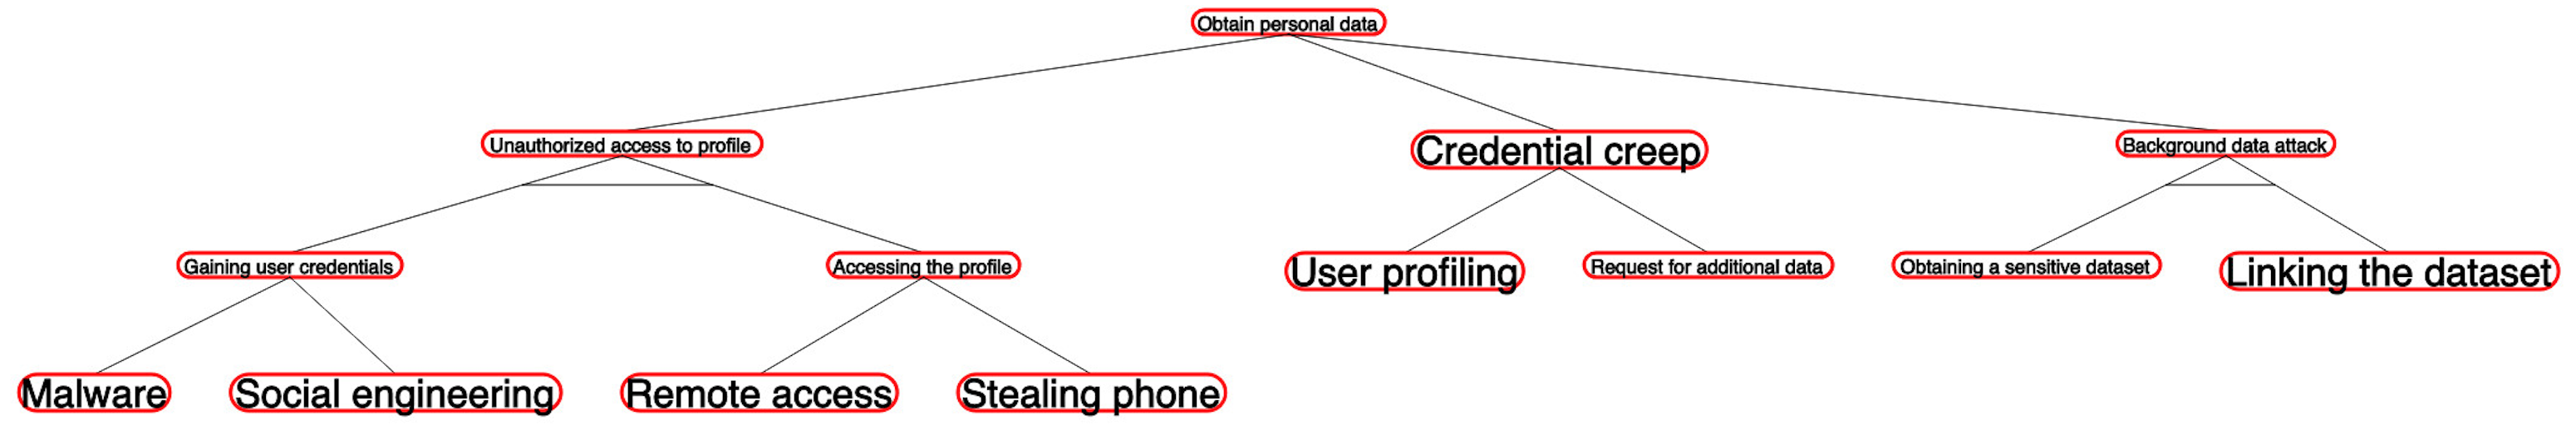
\includegraphics[width=\linewidth]{img/TargetAT.png}
    \caption{An attack tree adapted from Naik \etal~\cite{naikEvaluationPotentialAttack2022}. }
    \label{fig:tartgetAT}
\end{figure*}

We define attack trees to be a rooted acyclic structure with the following recursive definition adapted from Gadyatskaya~\etal~\cite{gadyatskayaRefinementAwareGenerationAttack2017}. 

\begin{definition} \label{def:attack-tree} An attack tree with $n$ nodes is defined as $T = T[n]\Delta(T[i],...,T[j])$ for some $i,j|1 \le i, i < j, j < n$. We define the $i\text{th}$ node according to left-right post-order number to be the following, $T[i] = b\Delta(T[j],...,T[k])$. We give $b$ to be some action within the attack scenario, which is the node label of $T[i]$. For clarity, we additionally refer to this label as $T[i].\text{label}$. We give $\Delta$ to be the refinement $\Delta = \AND|\OR$. For clarity and consistency, we refer to the refinement of a given node to be $T[i].\Delta$. Following the refinement, we have a list of nodes which are the children of $T[i]$, $T[j],...,T[k]$. This list of nodes can be empty, in the case of leaf nodes.
\end{definition}
      

Distance between data structures is not a new concept. Many works have explored the idea of ``distance'' between strings. In string edit distance, where the difference in strings is given my a min-cost path taken by either adding a character, removing a character or replacing a character. By fining the minimum cost needed to transform one string into another, a ``distance'' value can be given. As the higher cost a transformation, the further apart two strings must be \NS{cite all the string edit distance papers}.

Much of the work in this field has built upon work by Kuo-Chung Tai who suggested that the distance between trees is similar to several previous works comparing the differences in strings~\cite{tai_tree--tree_nodate}.


Zhang and Shasha have written the seminal work on tree edit distance~\cite{zhang_simple_1989}. In their work, they describe a simple algorithm for calculating the distance between two trees. This algorithm is based on the idea of a \textit{forest} distance, which is the distance between two forests. A forest is possible disjoint a collection of trees, though a forest can consist of a single tree. The distance between two forests is the minimum cost of transforming one forest into another. This is calculated by finding the minimum cost of transforming each tree in the first forest into each tree in the second forest. This is done recursively until the minimum cost of transforming each node in the first tree into each node in the second tree is found. The minimum cost of transforming the first tree into the second tree is then given as the optimal \emph{tree edit distance} between two trees. This edit distance is given as both a value, the cost of the sequence of edits, as well as the sequence of edits itself. This sequence of edits has 3 possible operations.

In the Zhang and Shasha algorithm the three possibilities for an edit operation between individual nodes are, (i) a node must be added, (ii) a node must be removed, or (iii) a node must be replaced~\cite{zhang_simple_1989}. Each of these operations has a cost 




\section{Related Work}

Tree Edit Distance is not a new computational challenge. However, most of the development on tree edit distance focuses calculation optimization. As shown by Zhang~\etal, the tree edit distance problem for unordered trees is an \textit{NP}-Complete problem~\cite{zhang_editing_1992}. As such, the develop of novel optimal calculation strategies is necessary to enable comparison of larger tree structures. Zhang and Shasha proposed a commonly cited simple algorithm for calculating tree edit distance~\cite{zhang_simple_1989}. We use this algorithm in this paper as it is a common strategy for implementing and testing extensions to tree edit distance. As such, optimizations based on the Zhang and Shasha algorithm can be applied to our methodology as we show in section \NS{When I write that section, I'll reference it here}.

Tree edit distance, like string edit distance, has a wide array of applications. Just as string edit distance has been used to compare sequences of DNA \NS{cite},
